% RECOMB 2027 manuscript using the optional Springer LLNCS class.
% Call for papers: 10 pages of main text excluding the bibliography, with an
% additional title page permitted; publicly accessible, documented source code
% is required for new software or analysis methods.
% Deadlines: abstract registration October 28, full paper November 4.
% Do not replace the LLNCS class or adjust layout just to shorten the paper.
\documentclass[10pt,letterpaper,runningheads]{llncs}
\usepackage[margin=1in]{geometry}
\usepackage[T1]{fontenc}
\usepackage{amsmath,amssymb}
\usepackage{booktabs}
\usepackage{graphicx}
\usepackage{xcolor}
\usepackage[hidelinks]{hyperref}
% Let the repository URL break across lines instead of running into the margin.
\usepackage{xurl}
\usepackage{refcount}
\usepackage{tikz}
\usetikzlibrary{patterns,arrows.meta}

% Keep captions, abstract, tables, and footnotes at the 10pt submission minimum.
\renewcommand{\small}{\fontsize{10}{12}\selectfont}
\renewcommand{\footnotesize}{\fontsize{10}{12}\selectfont}

\newcommand{\stl}{\textsc{stl}}
\newcommand{\mt}{\textsc{mt}}
\newcommand{\pooled}{\textsc{pooled}}
\newcommand{\simarm}{\textsc{sim}}
\newcommand{\rnd}{\textsc{rand}}
\newcommand{\auxtop}{\texttt{aux\_top}}
\newcommand{\auxnn}{\texttt{aux\_scaffold\_nn}}
\newcommand{\maxmin}{\texttt{maxmin}}
\newcommand{\rhoeff}{\rho_{\mathrm{eff}}}
\newcommand{\mtzero}{\textsc{mt}$_{r=0}$}

% Required: copy your actual generated summary files into generated/.
% Do NOT substitute example numbers in your submitted manuscript.
% Generated by scripts/summaries.py -- do not edit.
% Each macro is rendered from the same summary record that
% produces the corresponding table cell.

\newcommand{\valMtUniform}{$+11.49$}
\newcommand{\semMtUniform}{$3.25$}
\newcommand{\ciMtUniform}{$[+3.14,+19.84]$}
\newcommand{\nMtUniform}{6}
\newcommand{\posMtUniform}{6/6}
\newcommand{\pMtUniform}{$0.031$}

\newcommand{\valMtWithheld}{$+9.37$}
\newcommand{\semMtWithheld}{$2.99$}
\newcommand{\ciMtWithheld}{$[+1.67,+17.06]$}
\newcommand{\nMtWithheld}{6}
\newcommand{\posMtWithheld}{6/6}
\newcommand{\pMtWithheld}{$0.031$}

\newcommand{\valMtDesignChange}{$+2.12$}
\newcommand{\semMtDesignChange}{$1.04$}
\newcommand{\ciMtDesignChange}{$[-0.56,+4.80]$}
\newcommand{\nMtDesignChange}{6}
\newcommand{\posMtDesignChange}{4/6}
\newcommand{\pMtDesignChange}{$0.156$}

\newcommand{\valMtDesignChangeCell}{$+2.12$}
\newcommand{\semMtDesignChangeCell}{$1.02$}
\newcommand{\ciMtDesignChangeCell}{$[-0.12,+4.37]$}
\newcommand{\nMtDesignChangeCell}{12}
\newcommand{\posMtDesignChangeCell}{9/12}
\newcommand{\pMtDesignChangeCell}{$0.055$}

\newcommand{\valPooledUniform}{$+3.16$}
\newcommand{\semPooledUniform}{$5.14$}
\newcommand{\ciPooledUniform}{$[-10.06,+16.37]$}
\newcommand{\nPooledUniform}{6}
\newcommand{\posPooledUniform}{4/6}
\newcommand{\pPooledUniform}{$0.438$}

\newcommand{\valPooledWithheld}{$+8.89$}
\newcommand{\semPooledWithheld}{$4.74$}
\newcommand{\ciPooledWithheld}{$[-3.29,+21.06]$}
\newcommand{\nPooledWithheld}{6}
\newcommand{\posPooledWithheld}{5/6}
\newcommand{\pPooledWithheld}{$0.156$}

\newcommand{\valPooledDesignChange}{$-5.73$}
\newcommand{\semPooledDesignChange}{$2.01$}
\newcommand{\ciPooledDesignChange}{$[-10.91,-0.55]$}
\newcommand{\nPooledDesignChange}{6}
\newcommand{\posPooledDesignChange}{0/6}
\newcommand{\pPooledDesignChange}{$0.031$}

\newcommand{\valPooledDesignChangeCell}{$-5.73$}
\newcommand{\semPooledDesignChangeCell}{$1.56$}
\newcommand{\ciPooledDesignChangeCell}{$[-9.16,-2.29]$}
\newcommand{\nPooledDesignChangeCell}{12}
\newcommand{\posPooledDesignChangeCell}{1/12}
\newcommand{\pPooledDesignChangeCell}{$0.003$}

\newcommand{\valNullJakMtRand}{$+2.03$}
\newcommand{\semNullJakMtRand}{$0.86$}
\newcommand{\ciNullJakMtRand}{$[+0.33,+3.74]$}
\newcommand{\nNullJakMtRand}{128}
\newcommand{\posNullJakMtRand}{40/128}
\newcommand{\pNullJakMtRand}{$0.020$}

\newcommand{\valNullJakPooledRand}{$+0.55$}
\newcommand{\semNullJakPooledRand}{$0.94$}
\newcommand{\ciNullJakPooledRand}{$[-1.31,+2.40]$}
\newcommand{\nNullJakPooledRand}{128}
\newcommand{\posNullJakPooledRand}{37/128}
\newcommand{\pNullJakPooledRand}{$0.560$}

\newcommand{\valNullJakMtReal}{$+7.66$}
\newcommand{\semNullJakMtReal}{$0.99$}
\newcommand{\ciNullJakMtReal}{$[+5.70,+9.61]$}
\newcommand{\nNullJakMtReal}{128}
\newcommand{\posNullJakMtReal}{63/128}
\newcommand{\pNullJakMtReal}{$0.000$}

\newcommand{\valNullJakPooledReal}{$+5.70$}
\newcommand{\semNullJakPooledReal}{$1.01$}
\newcommand{\ciNullJakPooledReal}{$[+3.70,+7.71]$}
\newcommand{\nNullJakPooledReal}{128}
\newcommand{\posNullJakPooledReal}{54/128}
\newcommand{\pNullJakPooledReal}{$0.000$}

\newcommand{\valNullCypMtRand}{$-0.47$}
\newcommand{\semNullCypMtRand}{$1.55$}
\newcommand{\ciNullCypMtRand}{$[-3.53,+2.60]$}
\newcommand{\nNullCypMtRand}{128}
\newcommand{\posNullCypMtRand}{33/128}
\newcommand{\pNullCypMtRand}{$0.763$}

\newcommand{\valNullCypPooledRand}{$+10.55$}
\newcommand{\semNullCypPooledRand}{$1.85$}
\newcommand{\ciNullCypPooledRand}{$[+6.89,+14.20]$}
\newcommand{\nNullCypPooledRand}{128}
\newcommand{\posNullCypPooledRand}{78/128}
\newcommand{\pNullCypPooledRand}{$0.000$}

\newcommand{\valNullCypMtReal}{$+9.69$}
\newcommand{\semNullCypMtReal}{$1.50$}
\newcommand{\ciNullCypMtReal}{$[+6.71,+12.66]$}
\newcommand{\nNullCypMtReal}{128}
\newcommand{\posNullCypMtReal}{69/128}
\newcommand{\pNullCypMtReal}{$0.000$}

\newcommand{\valNullCypPooledReal}{$+17.50$}
\newcommand{\semNullCypPooledReal}{$1.70$}
\newcommand{\ciNullCypPooledReal}{$[+14.14,+20.86]$}
\newcommand{\nNullCypPooledReal}{128}
\newcommand{\posNullCypPooledReal}{94/128}
\newcommand{\pNullCypPooledReal}{$0.000$}

\newcommand{\valMechJakMtRZero}{$+2.03$}
\newcommand{\semMechJakMtRZero}{$0.83$}
\newcommand{\ciMechJakMtRZero}{$[+0.38,+3.68]$}
\newcommand{\nMechJakMtRZero}{128}
\newcommand{\posMechJakMtRZero}{40/128}
\newcommand{\pMechJakMtRZero}{$0.016$}

\newcommand{\valMechJakMt}{$+2.03$}
\newcommand{\semMechJakMt}{$0.86$}
\newcommand{\ciMechJakMt}{$[+0.33,+3.74]$}
\newcommand{\nMechJakMt}{128}
\newcommand{\posMechJakMt}{40/128}
\newcommand{\pMechJakMt}{$0.020$}

\newcommand{\valMechJakPooled}{$+0.55$}
\newcommand{\semMechJakPooled}{$0.94$}
\newcommand{\ciMechJakPooled}{$[-1.31,+2.40]$}
\newcommand{\nMechJakPooled}{128}
\newcommand{\posMechJakPooled}{37/128}
\newcommand{\pMechJakPooled}{$0.560$}

\newcommand{\valMechCypMtRZero}{$+0.08$}
\newcommand{\semMechCypMtRZero}{$1.25$}
\newcommand{\ciMechCypMtRZero}{$[-2.40,+2.56]$}
\newcommand{\nMechCypMtRZero}{128}
\newcommand{\posMechCypMtRZero}{31/128}
\newcommand{\pMechCypMtRZero}{$0.950$}

\newcommand{\valMechCypMt}{$-0.47$}
\newcommand{\semMechCypMt}{$1.55$}
\newcommand{\ciMechCypMt}{$[-3.53,+2.60]$}
\newcommand{\nMechCypMt}{128}
\newcommand{\posMechCypMt}{33/128}
\newcommand{\pMechCypMt}{$0.763$}

\newcommand{\valMechCypPooled}{$+10.55$}
\newcommand{\semMechCypPooled}{$1.85$}
\newcommand{\ciMechCypPooled}{$[+6.89,+14.20]$}
\newcommand{\nMechCypPooled}{128}
\newcommand{\posMechCypPooled}{78/128}
\newcommand{\pMechCypPooled}{$0.000$}

\newcommand{\valScaleMatchedJak}{$+2.34$}
\newcommand{\semScaleMatchedJak}{$0.73$}
\newcommand{\ciScaleMatchedJak}{$[+0.90,+3.79]$}
\newcommand{\nScaleMatchedJak}{128}
\newcommand{\posScaleMatchedJak}{41/128}
\newcommand{\pScaleMatchedJak}{$0.002$}

\newcommand{\valScaleMatchedCyp}{$-0.23$}
\newcommand{\semScaleMatchedCyp}{$0.67$}
\newcommand{\ciScaleMatchedCyp}{$[-1.56,+1.09]$}
\newcommand{\nScaleMatchedCyp}{128}
\newcommand{\posScaleMatchedCyp}{15/128}
\newcommand{\pScaleMatchedCyp}{$0.727$}


% Generated by scripts/family_table.py -- do not edit.
\newcommand{\rhoPooledCoupling}{$+0.886$}
\newcommand{\pPooledCoupling}{$0.019$}
\newcommand{\rhoMtCoupling}{$+0.771$}
\newcommand{\pMtCoupling}{$0.072$}
\newcommand{\nCouplingFamilies}{6}

% Generated by scripts/avoidance_calibration.py -- do not edit.
% The auxiliary-value-free avoidance control (C4), measured at the
% penalty W calibrated to the pooled model's own selection ratio.

\newcommand{\avoidCoverageFifty}{$45\%$}
\newcommand{\avoidHistoryFifty}{50}
\newcommand{\avoidWFifty}{$0.2274$}
\newcommand{\avoidTargetRatioFifty}{$0.2177$}
\newcommand{\avoidAchievedRatioFifty}{$0.2146$}
\newcommand{\avoidCampaignsFifty}{128}
\newcommand{\avoidRecallWithheldFifty}{$+17.03$}
\newcommand{\avoidRecallUniformFifty}{$-5.31$}
\newcommand{\avoidRecallSwingFifty}{$+22.34$}
\newcommand{\avoidRecallFracFifty}{$77\%$}
\newcommand{\avoidAucSwingFifty}{$+0.1180$}
\newcommand{\avoidAucFracFifty}{$77\%$}
\newcommand{\pooledRecallSwingFifty}{$+29.06$}
\newcommand{\pooledRecallWithheldFifty}{$+10.55$}
\newcommand{\pooledRecallUniformFifty}{$-18.52$}

\newcommand{\avoidCoverageHundred}{$90\%$}
\newcommand{\avoidHistoryHundred}{100}
\newcommand{\avoidWHundred}{$0.3794$}
\newcommand{\avoidTargetRatioHundred}{$0.8199$}
\newcommand{\avoidAchievedRatioHundred}{$0.8177$}
\newcommand{\avoidCampaignsHundred}{128}
\newcommand{\avoidRecallWithheldHundred}{$+30.47$}
\newcommand{\avoidRecallUniformHundred}{$-3.05$}
\newcommand{\avoidRecallSwingHundred}{$+33.52$}
\newcommand{\avoidRecallFracHundred}{$73\%$}
\newcommand{\avoidAucSwingHundred}{$+0.3479$}
\newcommand{\avoidAucFracHundred}{$84\%$}
\newcommand{\pooledRecallSwingHundred}{$+46.02$}
\newcommand{\pooledRecallWithheldHundred}{$+22.97$}
\newcommand{\pooledRecallUniformHundred}{$-23.05$}

% Generated by scripts/family_inference_audit.py -- do not edit.
% Six-family null comparison under uniformly sampled histories.

\newcommand{\permMtUniform}{$+11.49$}
\newcommand{\permSemMtUniform}{$3.25$}
\newcommand{\permCiMtUniform}{$[+3.14,+19.84]$}
\newcommand{\permPosMtUniform}{6/6}
\newcommand{\permPMtUniform}{$0.031$}
\newcommand{\permPtMtUniform}{$0.017$}

\newcommand{\permMtUnderShuf}{$-1.37$}
\newcommand{\permSemMtUnderShuf}{$0.71$}
\newcommand{\permCiMtUnderShuf}{$[-3.20,+0.45]$}
\newcommand{\permPosMtUnderShuf}{1/6}
\newcommand{\permPMtUnderShuf}{$0.156$}
\newcommand{\permPtMtUnderShuf}{$0.111$}

\newcommand{\permMtGvalueShuf}{$+12.86$}
\newcommand{\permSemMtGvalueShuf}{$3.48$}
\newcommand{\permCiMtGvalueShuf}{$[+3.92,+21.81]$}
\newcommand{\permPosMtGvalueShuf}{6/6}
\newcommand{\permPMtGvalueShuf}{$0.031$}
\newcommand{\permPtMtGvalueShuf}{$0.014$}

\newcommand{\permMtUnderQZero}{$-0.66$}
\newcommand{\permSemMtUnderQZero}{$0.50$}
\newcommand{\permCiMtUnderQZero}{$[-1.94,+0.63]$}
\newcommand{\permPosMtUnderQZero}{2/6}
\newcommand{\permPMtUnderQZero}{$0.312$}
\newcommand{\permPtMtUnderQZero}{$0.245$}

\newcommand{\permMtGvalueQZero}{$+12.15$}
\newcommand{\permSemMtGvalueQZero}{$3.45$}
\newcommand{\permCiMtGvalueQZero}{$[+3.27,+21.03]$}
\newcommand{\permPosMtGvalueQZero}{6/6}
\newcommand{\permPMtGvalueQZero}{$0.031$}
\newcommand{\permPtMtGvalueQZero}{$0.017$}

\newcommand{\permMtNullDifference}{$+0.72$}
\newcommand{\permSemMtNullDifference}{$0.38$}
\newcommand{\permCiMtNullDifference}{$[-0.26,+1.69]$}
\newcommand{\permPosMtNullDifference}{4/6}
\newcommand{\permPMtNullDifference}{$0.156$}
\newcommand{\permPtMtNullDifference}{$0.117$}

\newcommand{\permPooledUniform}{$+3.16$}
\newcommand{\permSemPooledUniform}{$5.14$}
\newcommand{\permCiPooledUniform}{$[-10.06,+16.37]$}
\newcommand{\permPosPooledUniform}{4/6}
\newcommand{\permPPooledUniform}{$0.438$}
\newcommand{\permPtPooledUniform}{$0.566$}

\newcommand{\permPooledUnderShuf}{$-16.20$}
\newcommand{\permSemPooledUnderShuf}{$2.40$}
\newcommand{\permCiPooledUnderShuf}{$[-22.36,-10.03]$}
\newcommand{\permPosPooledUnderShuf}{0/6}
\newcommand{\permPPooledUnderShuf}{$0.031$}
\newcommand{\permPtPooledUnderShuf}{$0.001$}

\newcommand{\permPooledGvalueShuf}{$+19.36$}
\newcommand{\permSemPooledGvalueShuf}{$4.47$}
\newcommand{\permCiPooledGvalueShuf}{$[+7.86,+30.85]$}
\newcommand{\permPosPooledGvalueShuf}{6/6}
\newcommand{\permPPooledGvalueShuf}{$0.031$}
\newcommand{\permPtPooledGvalueShuf}{$0.008$}

\newcommand{\permPooledUnderQZero}{$-16.42$}
\newcommand{\permSemPooledUnderQZero}{$2.39$}
\newcommand{\permCiPooledUnderQZero}{$[-22.57,-10.27]$}
\newcommand{\permPosPooledUnderQZero}{0/6}
\newcommand{\permPPooledUnderQZero}{$0.031$}
\newcommand{\permPtPooledUnderQZero}{$0.001$}

\newcommand{\permPooledGvalueQZero}{$+19.58$}
\newcommand{\permSemPooledGvalueQZero}{$4.29$}
\newcommand{\permCiPooledGvalueQZero}{$[+8.56,+30.60]$}
\newcommand{\permPosPooledGvalueQZero}{6/6}
\newcommand{\permPPooledGvalueQZero}{$0.031$}
\newcommand{\permPtPooledGvalueQZero}{$0.006$}

\newcommand{\permPooledNullDifference}{$-0.22$}
\newcommand{\permSemPooledNullDifference}{$0.49$}
\newcommand{\permCiPooledNullDifference}{$[-1.49,+1.05]$}
\newcommand{\permPosPooledNullDifference}{3/6}
\newcommand{\permPPooledNullDifference}{$0.688$}
\newcommand{\permPtPooledNullDifference}{$0.672$}

\newcommand{\permPFloor}{$0.031$}

% Generated by scripts/summarize_crossed_auxiliary.py; do not edit.
\newcommand{\crossPrimary}{+12.67}
\newcommand{\crossPrimaryCi}{[+2.53,+22.81]}
\newcommand{\crossPrimaryPositive}{6}
\newcommand{\crossMeasuredGain}{+11.49}
\newcommand{\crossMeasuredGainCi}{[+3.14,+19.84]}
\newcommand{\crossMeasuredGainPositive}{6}
\newcommand{\crossPermutedGain}{-1.18}
\newcommand{\crossPermutedGainCi}{[-3.31,+0.96]}
\newcommand{\crossPermutedGainPositive}{2}
\newcommand{\crossResponseMeasuredFit}{+17.30}
\newcommand{\crossResponseMeasuredFitCi}{[+5.59,+29.02]}
\newcommand{\crossResponseMeasuredFitPositive}{6}
\newcommand{\crossResponsePermutedFit}{+4.95}
\newcommand{\crossResponsePermutedFitCi}{[-0.24,+10.14]}
\newcommand{\crossResponsePermutedFitPositive}{5}
\newcommand{\crossFitMeasuredResponse}{+7.72}
\newcommand{\crossFitMeasuredResponseCi}{[+1.42,+14.02]}
\newcommand{\crossFitMeasuredResponsePositive}{6}
\newcommand{\crossFitPermutedResponse}{-4.64}
\newcommand{\crossFitPermutedResponseCi}{[-8.96,-0.31]}
\newcommand{\crossFitPermutedResponsePositive}{0}
\newcommand{\crossInteraction}{+12.36}
\newcommand{\crossInteractionCi}{[+5.05,+19.67]}
\newcommand{\crossInteractionPositive}{6}
\newcommand{\crossPrimaryP}{0.03125}
\newcommand{\crossCampaigns}{128}
\newcommand{\crossStlAnchorSTLBatchHits}{0.622}
\newcommand{\crossStlAnchorMMBatchHits}{1.237}
\newcommand{\crossStlAnchorMPBatchHits}{0.368}
\newcommand{\crossStlAnchorPMBatchHits}{0.801}
\newcommand{\crossStlAnchorPPBatchHits}{0.523}
\newcommand{\crossMtAnchorSTLBatchHits}{0.514}
\newcommand{\crossMtAnchorMMBatchHits}{0.757}
\newcommand{\crossMtAnchorMPBatchHits}{0.310}
\newcommand{\crossMtAnchorPMBatchHits}{0.597}
\newcommand{\crossMtAnchorPPBatchHits}{0.441}


\title{When Does Auxiliary Data Really Help Molecular Bayesian Optimization?}
\titlerunning{When Does Auxiliary Data Help Molecular BO?}

% RECOMB 2027 review is single-blind; verify author details before submission.

\author{Thanh Tran\orcidID{0009-0008-8775-074X}}

\authorrunning{T. Tran}

\institute{
University of Texas at Arlington,
Arlington, TX, USA\\
\email{cxt5391@mavs.uta.edu}
}

\begin{document}
\maketitle

\begin{abstract}
Historical assays from related protein targets are often reused to guide
molecular Bayesian optimization (BO). A higher hit-recovery rate, however,
does not establish that the auxiliary activity values improved the search:
historical data also change GP parameter fitting, posterior conditioning,
and which compounds the acquisition function selects. We present a
four-control attribution protocol that separates these routes. The controls
permute auxiliary responses while holding their observed locations fixed,
cross the responses used for hyperparameter fitting against those entering
the posterior, rescale acquisition uncertainty, and vary the rule by which
historical compounds were sampled.

Applied to BindingDB libraries from six protein families, the protocol
shows that fitted multi-task BO gains $\crossMeasuredGain{}$ points of
Recall@10 over single-task BO under uniform histories, whereas the same
model with permuted auxiliary responses gains $\crossPermutedGain{}$.
Fitting and conditioning interact: fitting on measured responses helps when
the posterior is conditioned on measured values
($\crossFitMeasuredResponse{}$ points) and hurts when it is conditioned on
permuted values ($\crossFitPermutedResponse{}$ points), an interaction of
$\crossInteraction{}$ points that is positive in all six families. Because
reconditioning at a shared state leaves predictive variance unchanged,
matched-state replays attribute the changed batch to the posterior mean
alone. Full pooling instead responds to how historical compounds were
sampled, and a policy that avoids them without reading any auxiliary
response reproduces most of that sensitivity.

The protocol separates gains that require auxiliary response correspondence
from changes in fitting and selection that do not, and yields a concrete
reporting set for assay-transfer benchmarks.

\end{abstract}

% RECOMB permits an additional page containing the title, authors, and abstract.
\clearpage
\label{page:main-start}

\section{Introduction}
\label{sec:intro}

Screening a molecular library for compounds active against a target protein
is expensive, so each assay choice matters. Bayesian optimization (BO)
selects compounds using a surrogate model and an acquisition
function~\cite{jones1998ego,shahriari2016taking}. Early in a campaign,
only a few primary-target measurements are available. Assays from related
targets provide a possible source of information, and multi-task BO can
use them without increasing the number of new primary-target assays~\cite{zhao2020multitask,swersky2013multitask}.

An improvement in hit recovery is not necessarily an improvement caused by
transfer of activity values. Auxiliary responses influence both GP
hyperparameter fitting and posterior conditioning. Historical compound
locations can also change the acquisition policy, even when their activity
values are uninformative. A comparison based only on final recall cannot
separate these possibilities.

\paragraph{Related work.}
Molecular BO and active learning prioritize compound measurements under
limited screening budgets~\cite{graff2021accelerating,gao2022pmo}, and
multifidelity BO combines measurements of different costs or
accuracies~\cite{mcdonald2025multifidelity}; our auxiliary data instead
consist of existing assays on related protein targets. Multi-task GPs link
targets through a shared compound kernel and a task covariance
matrix~\cite{bonilla2007multitask,swersky2013multitask}, and HyperBO learns
GP priors from earlier tasks~\cite{wang2024hyperbo}. Two recent results
motivate the present question. Sedgwick et al.~\cite{sedgwick2025transfer}
distinguish transfer through shared GP parameters from transfer through
correlated function values. Hvarfner et al.~\cite{hvarfner2026pitfalls}
show that per-task standardization and limited design overlap leave the
task correlation itself weakly identified, and propose co-locating part of
the source and target designs as a remedy; their evaluation uses synthetic
and hyperparameter-tuning benchmarks. Neither randomizes auxiliary
responses at fixed locations, crosses the fitting and conditioning
channels, nor varies the historical sampling rule. Our sampling control
also bears on the co-location remedy: a pooled model selects historically
assayed compounds well below their share of the library, so overlap
imposed by design can be undone by the acquisition policy.

We test the role of auxiliary response--compound correspondence by changing
which responses enter fitting and which enter posterior conditioning.
For six BindingDB protein families, we cross measured responses with
within-target permutations while holding historical observation locations
fixed (Fig.~\ref{fig:design}). Sequential campaigns capture the resulting
feedback through subsequent assay choices. Replays at shared primary-target
observations isolate the next-batch decisions. We also test whether changes
in acquisition uncertainty or in historical compound selection reproduce
parts of the observed gains.

\begin{figure}[t]
\centering
% Drawn in TikZ: vector, no external file, inherits the document font.
\small
% ---- (a) observation matrix -------------------------------------------
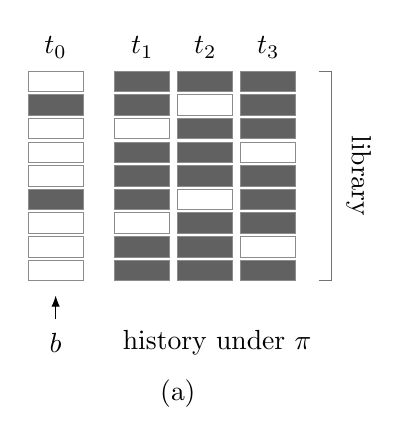
\begin{tikzpicture}[x=1mm,y=1mm,
    cell/.style={draw=black!45,line width=0.3pt},
    obs/.style={cell,fill=black!62}]
  \node at (3.5,3) {$t_0$};
  \node at (14.5,3) {$t_1$};
  \node at (22.5,3) {$t_2$};
  \node at (30.5,3) {$t_3$};
  \foreach \r in {0,...,8}{
    \draw[cell] (0,{-3*\r}) rectangle (7,{-3*\r-2.6});
    \draw[cell] (11,{-3*\r}) rectangle (18,{-3*\r-2.6});
    \draw[cell] (19,{-3*\r}) rectangle (26,{-3*\r-2.6});
    \draw[cell] (27,{-3*\r}) rectangle (34,{-3*\r-2.6});}
  \foreach \r in {1,5}{\draw[obs] (0,{-3*\r}) rectangle (7,{-3*\r-2.6});}
  \foreach \r in {0,1,3,4,5,7,8}{\draw[obs] (11,{-3*\r}) rectangle (18,{-3*\r-2.6});}
  \foreach \r in {0,2,3,4,6,7,8}{\draw[obs] (19,{-3*\r}) rectangle (26,{-3*\r-2.6});}
  \foreach \r in {0,1,2,4,5,6,8}{\draw[obs] (27,{-3*\r}) rectangle (34,{-3*\r-2.6});}
  \draw[black!55,line width=0.3pt] (37,0) -- (38.5,0) -- (38.5,-26.6) -- (37,-26.6);
  \node[rotate=-90] at (42,-13.3) {library};
  \draw[-{Latex[length=1.4mm]},line width=0.35pt] (3.5,-31.5) -- (3.5,-28.5);
  \node at (3.5,-34.5) {$b$};
  \node at (24,-34.5) {history under $\pi$};
  \node at (19,-41) {(a)};
\end{tikzpicture}\hfill
% ---- (b) within-target permutation ------------------------------------
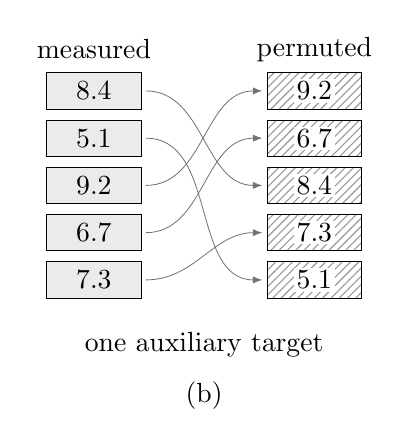
\begin{tikzpicture}[x=1mm,y=1mm,
    box/.style={draw=black,line width=0.35pt}]
  \node at (6,3) {measured};
  \node at (34,3) {permuted};
  \foreach \r/\v in {0/8.4,1/5.1,2/9.2,3/6.7,4/7.3}{
    \draw[box,fill=black!8] (0,{-6*\r}) rectangle (12,{-6*\r-4.6});
    \node at (6,{-6*\r-2.3}) {\v};}
  \foreach \r/\v in {0/9.2,1/6.7,2/8.4,3/7.3,4/5.1}{
    \draw[box,pattern=north east lines,pattern color=black!40]
      (28,{-6*\r}) rectangle (40,{-6*\r-4.6});
    \node[fill=white,inner sep=0.35mm] at (34,{-6*\r-2.3}) {\v};}
  \foreach \s/\t in {0/2,1/4,2/0,3/1,4/3}{
    \draw[-{Latex[length=1.2mm]},black!55,line width=0.3pt]
      (12.6,{-6*\s-2.3}) to[out=0,in=180] (27.4,{-6*\t-2.3});}
  \node at (20,-34.5) {one auxiliary target};
  \node at (20,-41) {(b)};
\end{tikzpicture}\hfill
% ---- (c) fitting x conditioning ---------------------------------------
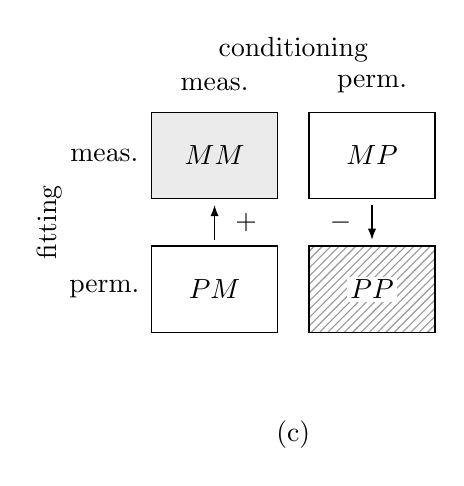
\begin{tikzpicture}[x=1mm,y=1mm,
    box/.style={draw=black,line width=0.4pt}]
  \node at (18,8) {conditioning};
  \node at (8,3.5) {meas.};
  \node at (28,3.5) {perm.};
  \node[rotate=90] at (-13,-14) {fitting};
  \node at (-6,-5.5) {meas.};
  \node at (-6,-22.5) {perm.};
  \draw[box,fill=black!8] (0,0) rectangle (16,-11);
  \draw[box] (20,0) rectangle (36,-11);
  \draw[box] (0,-17) rectangle (16,-28);
  \draw[box,pattern=north east lines,pattern color=black!40] (20,-17) rectangle (36,-28);
  \node at (8,-5.5) {$MM$};
  \node at (28,-5.5) {$MP$};
  \node at (8,-22.5) {$PM$};
  \node[fill=white,inner sep=0.4mm] at (28,-22.5) {$PP$};
  \draw[-{Latex[length=1.4mm]},line width=0.4pt] (8,-16.2) -- (8,-11.8);
  \node at (12,-14) {$+$};
  \draw[-{Latex[length=1.4mm]},line width=0.4pt] (28,-11.8) -- (28,-16.2);
  \node at (24,-14) {$-$};
  \node at (18,-41) {(c)};
\end{tikzpicture}
\caption{The crossed design. (a) Each family has one primary target $t_0$
and three auxiliary targets. The budget $b$ limits observations on $t_0$,
while auxiliary history is dense; $\pi$ sets which library compounds that
history covers. (b) Permutation reassigns responses to compounds within an
auxiliary target. The locations and the response multiset are unchanged.
(c) The responses used for fitting are crossed with the responses used for
the posterior, at identical history. The fitting effect takes opposite
signs in the two columns ($MM-PM$ against $MP-PP$);
Table~\ref{tab:crossed} gives the values.}
\label{fig:design}
\end{figure}

Fitting and conditioning do not act independently: parameters fitted on
measured auxiliary responses help recall with measured conditioning values
but reduce it with permuted values. At a fixed fitted GP and shared
observations, measured versus permuted conditioning selects different
compounds without changing predictive variance. Separately, full pooling
responds strongly to the historical sampling rule. These comparisons
locate several sources of apparent transfer gains that final recall would
otherwise combine.

\paragraph{Contributions.}
\begin{enumerate}
\item \textbf{An attribution protocol for auxiliary assay reuse.} We define
four controls that separate the routes by which historical assays change a
campaign: response correspondence (C1), its interaction with hyperparameter
fitting (C2), acquisition uncertainty (C3), and historical compound
selection (C4). Response randomization is established for validating
molecular predictors~\cite{rucker2007yrandomization}; every control here
additionally holds the observed auxiliary \emph{locations} fixed, which
separates where history was measured from what it measured.

\item \textbf{A crossed fitting--conditioning design with an equal-variance
identity.} We cross the responses supplying fitted GP parameters with the
responses entering the posterior, retaining the donor's task coupling,
signal variance, noise ratio, normalization, and jitter. At a shared state
this reconditioning leaves GP predictive variance unchanged, so any change
in the proposed batch is attributable to the response-dependent posterior
mean. Prior work separates transfer through shared parameters from transfer
through correlated values~\cite{sedgwick2025transfer}; crossing the two
factorially measures the interaction that a one-at-a-time contrast cannot.

\item \textbf{Reporting requirements for assay-transfer benchmarks.} On six
BindingDB panels the interaction is $\crossInteraction{}$ points and
positive in all six families, so neither channel can be assessed alone.
C3 and C4 further show that a recall gain can be produced by rescaling
acquisition uncertainty or by avoiding historical compounds without reading
any auxiliary response. Section~\ref{sec:guidance} states the resulting
minimum reporting set.
\end{enumerate}

% SUBMISSION CHECK: as of 2026-10-19 this repository is still PRIVATE --
% an unauthenticated request returns HTTP 404. The sentence below states
% present availability, so switch the repository to public before compiling
% the submission PDF, and confirm the link resolves while signed out.
The repository at \url{https://github.com/uta-smile/Bo-Drug-discovery}
holds the code and the audited campaign records, and documents the build,
the experiment protocol, and the commands that regenerate every number
reported here.

\section{Methods}
\label{sec:framework}

We state the optimization setting, surrogate models, and evaluation
protocol, then define the four controls. C1 tests whether
response--compound correspondence matters at all; C2 crosses that
correspondence with GP fitting and is the primary analysis; C3 and C4 test
acquisition uncertainty and historical selection as alternative
explanations for the same recall gain.

\subsection{Setting, Models, and Acquisition}
\label{sec:matrix}

We optimize over a fixed library $\mathcal M$ of compounds, with a primary
protein target $t_0$ and related targets $t_1,\ldots,t_{T-1}$. The
activity $y(m,t_j)$ is defined so that larger values are better. An
observation mask $M\in\{0,1\}^{N\times T}$ records which compound--target
pairs were assayed; we do not impute missing values.

Retrospective campaigns reveal a primary-target activity only when the
corresponding compound is selected. We score recovery of the ten most
active compounds \emph{within the constructed library}, not recovery over
all possible molecules.

Auxiliary assays have already been collected in the main experiments and
do not consume the prospective primary-target budget. Each new
compound--target evaluation counts as one assay, and all new assays are
assigned to $t_0$. We study assay allocation separately in
Supplement~S3.

\label{sec:models}
An observed pair gives the training example
$((\mathbf{x}_m,t_j),y(m,t_j))$; compounds may have distinct responses at
different targets. Molecular inputs are fixed 2048-bit ECFP4
fingerprints~\cite{rogers2010ecfp,rdkit} with a Tanimoto kernel. We do
not use learned compound features or protein sequence or structure
features. The task covariance matrix provides the only cross-target
coupling.

We compare three GP surrogates. Single-task BO (\stl{}) trains only on
the primary target. Fitted multi-task BO (\mt{}) includes primary and
auxiliary measurements and estimates their coupling. Fully pooled BO
(\pooled{}) treats the targets as completely coupled.

For the multi-task model,
\[
k\big((m,a),(m',b)\big)
= k_{\mathrm{Tanimoto}}(m,m')B_{ab},\qquad
B=(1-r)I+r\mathbf{1}\mathbf{1}^{\top}.
\]
The single parameter $r$ sets the correlation between distinct targets:
$r=0$ removes direct cross-target covariance, whereas $r=1$ imposes
complete coupling. We select $r$ by marginal likelihood over the fixed
grid specified in Supplement~S1.1.

Kernel and noise hyperparameters are fitted jointly on primary and
auxiliary observations; each target's responses are standardized
separately. Full pooling therefore assumes a shared function on the
standardized activity scale. Even when $r=0$, auxiliary observations can
affect the shared hyperparameter estimates. We examine this possibility
with the covariance-free control (\mtzero{}); Supplement~S1 gives the GP
fitting details.

We select compounds by expected improvement (EI) relative to the best
primary-target activity observed so far, with improvement offset
$\xi=0.01$. EI depends on posterior mean and variance, so a model may
change screening decisions without improving activity predictions.

Campaigns begin with ten primary-target observations. We then acquire
batches of ten compounds using the highest EI scores without replacement.
The posterior is fixed within a batch and refitted after the batch is
observed; ties are broken randomly. A final partial batch respects the
assay budget. All methods use EI unless an acquisition control explicitly
changes its uncertainty input.

\subsection{Data, Metrics, and Inference}
\label{sec:setup}

We use BindingDB activity data~\cite{bindingdb2016} for six protein
families: JAK, CYP, DPP, HDAC, MMP, and PI3K. Each panel contains four
protein targets, and we retain compounds measured against all four. This
complete-panel requirement lets us vary historical observations without
confounding their sampling locations with unmeasured assay outcomes.
Each target serves once as the primary task, with the other three as
auxiliary targets. All six families enter the crossed evaluation; JAK and
CYP also enter the detailed acquisition and sampling analyses.

Removing reporting-limit artifacts leaves 904 compounds in JAK, 590 in
PI3K, 378 in HDAC, 335 in CYP, 300 in DPP, and 248 in MMP. These are
small libraries, particularly for top-10 recall. Target identifiers,
panel composition, and pairwise activity correlations are reported in
Supplement~S1.3. We retain recorded activities without imputation,
convert IC$_{50}$ to pIC$_{50}$ where appropriate, and exclude
reporting-limit artifacts (Supplement~S1). Assay-allocation and
initial-selection experiments appear in Supplements~S3--S4.

At budget $b$, Recall@10 is the fraction of the library's ten most active compounds already evaluated on the primary target. If
$\mathcal H_{10}$ is that set and $\mathcal S_b$ is the set of primary-target
compounds evaluated by budget $b$, then
\[
\operatorname{Recall@10}(b)
=\frac{|\mathcal S_b\cap\mathcal H_{10}|}{10}.
\]
We report gains over single-task BO in percentage points. For the
initial-design experiments we also report area under the recall curve,
which accounts for when hits are found.

The crossed evaluation uses 32 repeats for each of four primary targets
at two assay budgets per family. Each auxiliary target contributes 50
historical observations. Methods share the same starting observations,
historical samples, and assay budgets. Repeats measure variation within
these constructed panels, not independent biological replication. The
budgets within a family also share a historical draw, as verified by
index hashes (Supplement~S6). To avoid treating those runs as independent
families, we average over primary targets and repeats within each budget,
then over the two budgets within each family. The Wilcoxon signed-rank
test is applied to the resulting six family-level effects. We report
effect sizes, confidence intervals, and counts of positive families; the
smallest attainable two-sided $p$-value with $n=6$ is $0.03125$.

\subsection{The Four Controls}
\label{sec:method}
\label{sec:method-controls}

An auxiliary history consists of observed locations
$\mathcal L=\{(m,t_j):M_{mj}=1,\ j\geq1\}$, their responses
$y_{\mathrm{aux}}$, and a sampling policy $\pi$. The controls below compare
model behavior and screening policies; they do not identify unique
biological mechanisms or divide a total recall gain into independent
causal shares.

\paragraph{C1. Auxiliary-response randomization.}
We change auxiliary responses without changing primary-target responses
or historical observation locations. Within each auxiliary target, a
permutation preserves the values and empirical response distribution in
its sampled history while breaking their correspondence to compounds.
We sample locations first and use one fixed permutation per target and
repeat. A separate Gaussian-noise experiment interpolates between
measured responses ($q=1$) and randomized responses ($q=0$); noise is
regenerated for each held-out target and repeat (Supplement~S1.2).
Unlike permutation, Gaussian randomization does not preserve the
observed response distribution. We apply both controls to six families
with uniform histories, shared initial designs, and matched historical
locations, following the logic of molecular response-randomization
tests~\cite{rucker2007yrandomization}. Dataset composition and
cross-target relationships also affect how biological optimization
benchmarks should be read~\cite{wittmann2021informed,leakage2026};
permuting at fixed locations leaves the library and the historical
coverage untouched, so neither factor can account for a C1 effect.

\paragraph{C2. Response correspondence and joint fitting.}
At every selection round we fit two multi-task GPs on the same primary
observations and historical compound locations. One donor uses measured
auxiliary responses ($M$); the other uses their within-history
permutations ($P$). We then cross the donor fit with the responses used
for posterior conditioning. The four policies are $MM$, $MP$, $PM$, and
$PP$, where the first letter names the fit and the second names the
conditioning responses. Reconditioning retains the donor's task
coupling, signal variance, noise ratio, normalization transforms, and
numerical jitter. Each sequential policy refits donors using the
observations on its own trajectory.

$MM$ and $PP$ are ordinary measured- and permuted-response multi-task
BO, respectively. At a shared state, changing the conditioning values
with all fit parameters and observation locations fixed leaves GP
predictive variance unchanged; $MM$ versus $MP$ therefore changes the
response-dependent mean without changing variance. $MM$ versus $PM$
instead changes the fitted parameters while keeping measured
conditioning values. These equal-variance claims apply only to
shared-state comparisons, not to campaigns following different
trajectories.

We evaluate all four policies in sequential campaigns and in next-batch
replays at shared single-task and $MM$ states. In the replays, primary
observations are identical across conditions. In the campaigns, different
selections change subsequent observations. Note that $MP$ retains
response information in its measured-response donor, even though it
conditions on a permutation; it is not a response-free control. The
covariance-free case (\mtzero{}) is distinct: when $r=0$ and the
remaining parameters are fixed to their single-task values, the
single-task posterior is recovered. Details and the earlier JAK
comparison appear in Supplement~S2.

\paragraph{C3. Uncertainty-adjusted acquisition.}
We retain single-task data and predicted means but multiply the
predictive standard deviation used by EI by a constant:
\[
\widetilde{\sigma}(m)=c\,\sigma_{\stl}(m).
\]
We choose $c$ from the ratio of early predictive uncertainties under
fitted multi-task and single-task BO, without using recall to set it.
This intervention tests whether a change in exploration of that size can
reproduce a recall gain. It does not reproduce the full multi-task GP.

\paragraph{C4. Historical compound selection.}
Under \emph{uniform histories}, auxiliary compounds are sampled without
using their primary-target activities. Under \emph{withheld histories},
we exclude the primary target's true top-10 compounds. The latter uses
outcome information unavailable to a prospective sampling policy and is
used only as a stress test. Uniform histories are the primary evaluation.

A model that reduces uncertainty on historically assayed compounds may
select them less often under EI. That behavior could help under
withholding, where the best compounds are absent from history, but hurt
when uniform history includes some of them. We test the selection effect
without auxiliary response values by penalizing single-task EI on
historical compounds and comparing the resulting choices with full
pooling.

\section{Results}
\label{sec:results}

\subsection{Auxiliary Responses Contribute to Gains Under Uniform Histories}
\label{sec:res-null}

For uniform historical samples, fitted multi-task BO ($MM$) gains
$\crossMeasuredGain{}$ percentage points of recall over \stl{}. When
auxiliary responses are permuted before both fitting and conditioning
($PP$), the gain is $\crossPermutedGain{}$ points. The paired difference
is $\crossPrimary{}$ points (95\% CI $\crossPrimaryCi{}$), positive in
$\crossPrimaryPositive{}/6$ families ($p=\crossPrimaryP{}$).
These conditions retain the same historical compound locations and the
same multiset of response values within each auxiliary target; only
response--compound correspondence changes. There are
\crossCampaigns{} campaigns per family and budget, with the two budget
effects averaged within each family for inference. These runs reproduce
the original single-task and measured-response recall vectors. Detailed
results by budget and the earlier permutation tests are in
Supplement~S2.

\subsection{The Benefit of Response-Informed Fitting Depends on Posterior Conditioning}
\label{sec:res-mech}

Table~\ref{tab:crossed} reports the four crossed policies under uniform
histories. At the measured-response fit, replacing permuted with
measured conditioning responses changes recall by
$\crossResponseMeasuredFit{}$ points ($MM-MP$, 95\% CI
$\crossResponseMeasuredFitCi{}$). At the permuted-response fit, the
corresponding difference is $\crossResponsePermutedFit{}$ points
($PM-PP$, 95\% CI $\crossResponsePermutedFitCi{}$).

Holding conditioning responses measured while changing the fit gives
$\crossFitMeasuredResponse{}$ points ($MM-PM$, 95\% CI
$\crossFitMeasuredResponseCi{}$). With permuted conditioning, that
fitting contrast is $\crossFitPermutedResponse{}$ points ($MP-PP$,
95\% CI $\crossFitPermutedResponseCi{}$). The direction of the fitting
effect reverses with the conditioning responses: fitting on measured
values helps with measured conditioning but hurts with permuted
conditioning.

\begin{table}[htbp]
\caption{C2: Recall@10 gain over \stl{} (percentage points) under uniform
histories, averaged over the two budgets within each family. The first
letter identifies the response condition supplying fitted parameters; the
second identifies the conditioning responses ($M$: measured, $P$: permuted
within observed history). Each budget uses \crossCampaigns{} campaigns.}
\label{tab:crossed}
\centering
\begin{tabular}{lrrrr}
\toprule
Family & $\mathrm{MM}$ $-$ \stl{} & $\mathrm{MP}$ $-$ \stl{} & $\mathrm{PM}$ $-$ \stl{} & $\mathrm{PP}$ $-$ \stl{} \\
\midrule
JAK & $+6.37$ & $-2.07$ & $+4.49$ & $+1.99$ \\
CYP & $+15.51$ & $-13.09$ & $+9.18$ & $-2.38$ \\
DPP & $+3.87$ & $-1.76$ & $+0.70$ & $-1.21$ \\
HDAC & $+23.20$ & $-3.75$ & $+5.59$ & $-3.36$ \\
MMP & $+16.09$ & $-10.70$ & $+3.98$ & $-2.54$ \\
PI3K & $+3.91$ & $-3.52$ & $-1.33$ & $+0.43$ \\
\midrule
Mean & $+11.49$ & $-5.81$ & $+3.77$ & $-1.18$ \\
\bottomrule
\end{tabular}

\end{table}

\begin{figure}[htbp]
\centering
% Generated by scripts/make_crossed_figure.py; do not edit.
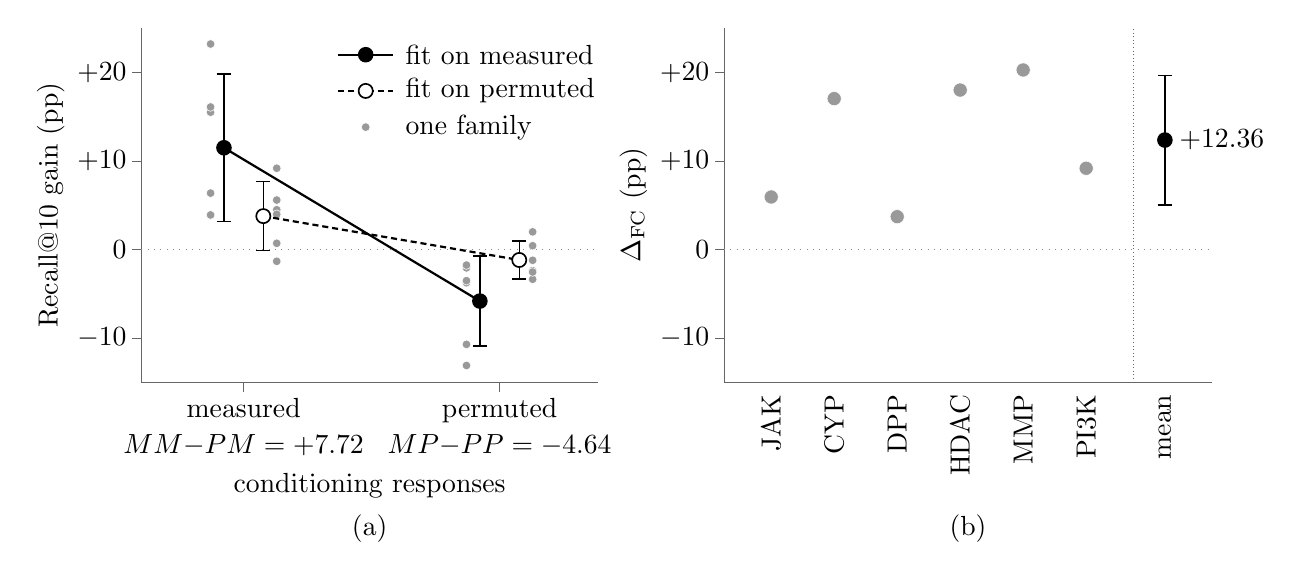
\begin{tikzpicture}[x=1mm,y=1mm,
    ax/.style={black!60,line width=0.3pt},
    zero/.style={black!45,line width=0.3pt,dotted},
    bar/.style={black,line width=0.5pt},
    fitM/.style={black,line width=0.8pt},
    fitP/.style={black,line width=0.8pt,dash pattern=on 2.2pt off 1.4pt},
    meanM/.style={fill=black,draw=black,line width=0.5pt},
    meanP/.style={fill=white,draw=black,line width=0.6pt},
    fam/.style={fill=black!40,draw=white,line width=0.2pt}]
  %% panel (a): Recall@10 gain by fitting x conditioning
  \draw[ax] (0.0,0.00) -- (0.0,45.00);
  \draw[ax] (0.0,5.62) -- (-1.2,5.62);
  \node[anchor=east,font=\small,inner sep=0.6mm] at (-1.2,5.62) {$-10$};
  \draw[ax] (0.0,16.88) -- (-1.2,16.88);
  \node[anchor=east,font=\small,inner sep=0.6mm] at (-1.2,16.88) {$0$};
  \draw[ax] (0.0,28.12) -- (-1.2,28.12);
  \node[anchor=east,font=\small,inner sep=0.6mm] at (-1.2,28.12) {$+10$};
  \draw[ax] (0.0,39.38) -- (-1.2,39.38);
  \node[anchor=east,font=\small,inner sep=0.6mm] at (-1.2,39.38) {$+20$};
  \node[rotate=90,font=\small] at (-11.5,22.50) {Recall@10 gain (pp)};
  \draw[zero] (0,16.88) -- (58.0,16.88);
  \draw[ax] (0,0.00) -- (58.0,0.00);
  \draw[ax] (13.0,0.00) -- (13.0,-1.20);
  \node[anchor=north,font=\small,inner sep=0pt] at (13.0,-2.00) {measured};
  \node[anchor=north,font=\small,inner sep=0pt] at (13.0,-6.50) {$MM{-}PM=+7.72$};
  \draw[ax] (45.5,0.00) -- (45.5,-1.20);
  \node[anchor=north,font=\small,inner sep=0pt] at (45.5,-2.00) {permuted};
  \node[anchor=north,font=\small,inner sep=0pt] at (45.5,-6.50) {$MP{-}PP=-4.64$};
  \node[anchor=north,font=\small,inner sep=0pt] at (29.0,-11.50) {conditioning responses};
  \fill[fam] (8.80,24.04) circle (0.55mm);
  \fill[fam] (8.80,34.32) circle (0.55mm);
  \fill[fam] (8.80,21.23) circle (0.55mm);
  \fill[fam] (8.80,42.98) circle (0.55mm);
  \fill[fam] (8.80,34.98) circle (0.55mm);
  \fill[fam] (8.80,21.27) circle (0.55mm);
  \fill[fam] (41.30,14.55) circle (0.55mm);
  \fill[fam] (41.30,2.15) circle (0.55mm);
  \fill[fam] (41.30,14.90) circle (0.55mm);
  \fill[fam] (41.30,12.66) circle (0.55mm);
  \fill[fam] (41.30,4.83) circle (0.55mm);
  \fill[fam] (41.30,12.92) circle (0.55mm);
  \fill[fam] (17.20,21.93) circle (0.55mm);
  \fill[fam] (17.20,27.20) circle (0.55mm);
  \fill[fam] (17.20,17.67) circle (0.55mm);
  \fill[fam] (17.20,23.16) circle (0.55mm);
  \fill[fam] (17.20,21.36) circle (0.55mm);
  \fill[fam] (17.20,15.38) circle (0.55mm);
  \fill[fam] (49.70,19.12) circle (0.55mm);
  \fill[fam] (49.70,14.19) circle (0.55mm);
  \fill[fam] (49.70,15.51) circle (0.55mm);
  \fill[fam] (49.70,13.10) circle (0.55mm);
  \fill[fam] (49.70,14.02) circle (0.55mm);
  \fill[fam] (49.70,17.36) circle (0.55mm);
  \draw[fitM] (10.50,29.80) -- (43.00,10.33);
  \draw[fitP] (15.50,21.12) -- (48.00,15.55);
  \draw[bar] (10.50,20.41) -- (10.50,39.19);
  \draw[bar] (9.60,20.41) -- (11.40,20.41);
  \draw[bar] (9.60,39.19) -- (11.40,39.19);
  \filldraw[meanM] (10.50,29.80) circle (0.9mm);
  \draw[bar] (43.00,4.63) -- (43.00,16.04);
  \draw[bar] (42.10,4.63) -- (43.90,4.63);
  \draw[bar] (42.10,16.04) -- (43.90,16.04);
  \filldraw[meanM] (43.00,10.33) circle (0.9mm);
  \draw[bar] (15.50,16.75) -- (15.50,25.49);
  \draw[bar] (14.60,16.75) -- (16.40,16.75);
  \draw[bar] (14.60,25.49) -- (16.40,25.49);
  \filldraw[meanP] (15.50,21.12) circle (0.9mm);
  \draw[bar] (48.00,13.15) -- (48.00,17.95);
  \draw[bar] (47.10,13.15) -- (48.90,13.15);
  \draw[bar] (47.10,17.95) -- (48.90,17.95);
  \filldraw[meanP] (48.00,15.55) circle (0.9mm);
  \draw[fitM] (25.0,41.62) -- (32.0,41.62);
  \filldraw[meanM] (28.5,41.62) circle (0.9mm);
  \node[anchor=west,font=\small,inner sep=0pt] at (33.5,41.62) {fit on measured};
  \draw[fitP] (25.0,37.02) -- (32.0,37.02);
  \filldraw[meanP] (28.5,37.02) circle (0.9mm);
  \node[anchor=west,font=\small,inner sep=0pt] at (33.5,37.02) {fit on permuted};
  \fill[fam] (28.5,32.42) circle (0.55mm);
  \node[anchor=west,font=\small,inner sep=0pt] at (33.5,32.42) {one family};
  \node[font=\small] at (29.0,-18.50) {(a)};
  %% panel (b): per-family interaction
  \draw[ax] (74.0,0.00) -- (74.0,45.00);
  \draw[ax] (74.0,5.62) -- (72.8,5.62);
  \node[anchor=east,font=\small,inner sep=0.6mm] at (72.8,5.62) {$-10$};
  \draw[ax] (74.0,16.88) -- (72.8,16.88);
  \node[anchor=east,font=\small,inner sep=0.6mm] at (72.8,16.88) {$0$};
  \draw[ax] (74.0,28.12) -- (72.8,28.12);
  \node[anchor=east,font=\small,inner sep=0.6mm] at (72.8,28.12) {$+10$};
  \draw[ax] (74.0,39.38) -- (72.8,39.38);
  \node[anchor=east,font=\small,inner sep=0.6mm] at (72.8,39.38) {$+20$};
  \node[rotate=90,font=\small] at (62.5,22.50) {$\Delta_{\mathrm{FC}}$ (pp)};
  \draw[zero] (74.0,16.88) -- (136.0,16.88);
  \draw[ax] (74.0,0.00) -- (136.0,0.00);
  \fill[fam] (80.0,23.55) circle (0.9mm);
  \node[rotate=90,anchor=east,font=\small,inner sep=0pt] at (80.0,-1.50) {JAK};
  \fill[fam] (88.0,36.04) circle (0.9mm);
  \node[rotate=90,anchor=east,font=\small,inner sep=0pt] at (88.0,-1.50) {CYP};
  \fill[fam] (96.0,21.05) circle (0.9mm);
  \node[rotate=90,anchor=east,font=\small,inner sep=0pt] at (96.0,-1.50) {DPP};
  \fill[fam] (104.0,37.13) circle (0.9mm);
  \node[rotate=90,anchor=east,font=\small,inner sep=0pt] at (104.0,-1.50) {HDAC};
  \fill[fam] (112.0,39.68) circle (0.9mm);
  \node[rotate=90,anchor=east,font=\small,inner sep=0pt] at (112.0,-1.50) {MMP};
  \fill[fam] (120.0,27.20) circle (0.9mm);
  \node[rotate=90,anchor=east,font=\small,inner sep=0pt] at (120.0,-1.50) {PI3K};
  \draw[ax,densely dotted] (126.0,0.00) -- (126.0,45.00);
  \draw[bar] (130.00,22.55) -- (130.00,39.00);
  \draw[bar] (129.10,22.55) -- (130.90,22.55);
  \draw[bar] (129.10,39.00) -- (130.90,39.00);
  \filldraw[meanM] (130.0,30.78) circle (0.9mm);
  \node[anchor=west,font=\small,inner sep=0pt] at (131.8,30.78) {$+12.36$};
  \node[rotate=90,anchor=east,font=\small,inner sep=0pt] at (130.0,-1.50) {mean};
  \node[font=\small] at (105.0,-18.50) {(b)};
\end{tikzpicture}

\caption{The fitting--conditioning interaction. (a) Recall@10 gain over
\stl{} as the conditioning responses change from measured to permuted,
for parameters fitted on measured responses (solid) and on permuted
responses (dashed). Thick marked lines are the six-family means; thin grey
lines are the individual families. The two vertical bars give the fitting
effect at each conditioning condition: $\crossFitMeasuredResponse{}$ points
with measured conditioning against $\crossFitPermutedResponse{}$ with
permuted conditioning, so the mean lines cross. (b) The interaction
$(MM-MP)-(PM-PP)$ for each family, with the six-family mean
$\crossInteraction{}$ (95\% CI $\crossInteractionCi{}$), positive in
$\crossInteractionPositive{}/6$ families.}
\label{fig:interaction}
\end{figure}

The prespecified descriptive contrasts give an interaction of
$\crossInteraction{}$ points (95\% CI $\crossInteractionCi{}$), positive in
every family (Fig.~\ref{fig:interaction}).
The shared-state replays distinguish this pattern from changes in
predictive variance. On single-task states, $MM$ and $MP$ propose
batches containing, on average, $\crossStlAnchorMMBatchHits{}$ and
$\crossStlAnchorMPBatchHits{}$ top-10 compounds, respectively. On shared
$MM$ states, the corresponding values are
$\crossMtAnchorMMBatchHits{}$ and $\crossMtAnchorMPBatchHits{}$.
Predictive variance is identical within each pair at every shared
state. The changed batch choices therefore arise from the
response-dependent means under a fixed fit. Replay measures immediate
proposals; it does not partition the final recall difference between
sequential campaigns. The covariance-free JAK diagnostic is reported in
Supplement~S2.

\subsection{Uncertainty Rescaling Reproduces the Randomized-Response JAK Gain but Not the CYP Effect}
\label{sec:res-exploration}

With covariance-free joint fitting, mean predictive standard deviation
falls from $0.643$ to $0.558$ on JAK and from $0.629$ to $0.522$ on CYP
(Supplement~S2). C3 asks whether a similar change in the uncertainty
input to EI can change discovery even without auxiliary training data.

Near 50 primary observations in the JAK campaigns, fitted \mt{} has
about $0.80$ times the predictive uncertainty of \stl{}. Rescaling the
single-task standard deviation in EI by $c=0.80$ gives a recall gain of
\valScaleMatchedJak{} $\pm$ \semScaleMatchedJak{} points. This is
comparable to the \valMechJakMt{}-point gain of \mt{} with randomized
auxiliary responses. When auxiliary responses are measured, \mt{}
exceeds the rescaled single-task policy by $5.31\pm0.91$ points.
This remaining difference is compatible with useful response
information, but the control does not estimate its isolated contribution.
Rescaling is a change to acquisition, not a test of GP calibration;
other calibration and chemical-isolation diagnostics appear in
Supplement~S2.

The CYP result is different. Among single-task scaling factors
$c\in[0.35,20]$, the largest gain is $+0.08$ points, versus a
\valMechCypPooled{}-point gain under pooling with randomized responses.
For these controls, uncertainty rescaling can reproduce the JAK gain
but not the CYP pooled-model effect.

\subsection{Historical Sampling Design Reverses the Benefit of Full Pooling}
\label{sec:res-design}

\paragraph{Outcome-informed withholding as a stress test.}
Withheld-history runs probe sensitivity to where historical assays were
collected. After auxiliary responses are randomized, \mt{} still gains
\valNullJakMtRand{} points on JAK, and \pooled{} gains
\valNullCypPooledRand{} points on CYP (Table~\ref{tab:null}). These
improvements do not require the original pairing of auxiliary activity
values with compounds. We therefore examine how the sampling rule
changes which compounds are selected.

\begin{table}[htbp]
\caption{C1: Change in top-10 recall relative to \stl{} (percentage points)
with randomized ($q=0$) or measured ($q=1$) auxiliary responses under
withheld histories. The observation locations are held fixed.
Mean $\pm$ SEM over $n=\nNullJakMtRand{}$ campaigns per comparison.}
\label{tab:null}
\centering
\small
\begin{tabular}{llcc}
\toprule
Block & Model vs.\ \stl{}
& $q=0$ (randomized)
& $q=1$ (measured) \\
\midrule

JAK & \mt{}
& \valNullJakMtRand{} $\pm$ \semNullJakMtRand{}
& \valNullJakMtReal{} $\pm$ \semNullJakMtReal{} \\

JAK & \pooled{}
& \valNullJakPooledRand{} $\pm$ \semNullJakPooledRand{}
& \valNullJakPooledReal{} $\pm$ \semNullJakPooledReal{} \\

CYP & \mt{}
& \valNullCypMtRand{} $\pm$ \semNullCypMtRand{}
& \valNullCypMtReal{} $\pm$ \semNullCypMtReal{} \\

CYP & \pooled{}
& \valNullCypPooledRand{} $\pm$ \semNullCypPooledRand{}
& \valNullCypPooledReal{} $\pm$ \semNullCypPooledReal{} \\

\bottomrule
\end{tabular}

\end{table}

Unlike fitted \mt{}, \pooled{} treats all targets as observations of
the same standardized activity function. Historical compounds can
therefore have lower predictive uncertainty and rank lower under EI.
On CYP with uniform histories, the frequency of selecting historical
compounds divided by their fraction of the library is $0.288$ under
\pooled{}, $0.542$ under \mt{}, and $0.972$ under \stl{}.
For \pooled{}, mean predictive standard deviation is $0.412$ on
historical compounds and $0.542$ elsewhere. This result concerns the
selected compounds, not necessarily the average EI within history.

Avoiding history is advantageous when history was constructed to exclude
the primary target's ten best compounds, but it may discard hits under
uniform sampling. On CYP with 300 historical entries and randomized
responses, the pooled recall gain changes from $+22.97$ points with
withholding to $-23.05$ points with uniform sampling, a roughly
46-point reversal. Under withholding, increasing history from 30 to
300 entries changes the gain from $-1.25$ to $+22.97$ points. At 150
historical entries under uniform sampling, permutation and Gaussian
randomization yield comparable effects ($-19.69$ and $-18.52$ points).
The original response--compound pairing is therefore not necessary for
this sampling sensitivity.

\paragraph{Auxiliary-value-free avoidance control.}
We apply a penalty $W$ to single-task EI at compounds appearing in
auxiliary history, without using their auxiliary responses. We calibrate
$W$ to reproduce the pooled policy's campaign-wide ratio of history
selection to library coverage. In separate CYP campaigns, the target
ratio \avoidTargetRatioHundred{} is matched within $0.003$
(\avoidAchievedRatioHundred{} at $W=\avoidWHundred{}$).
The penalty policy accounts for \avoidRecallFracHundred{} of the
pooled model's withheld-to-uniform recall change
(\avoidRecallSwingHundred{} versus \pooledRecallSwingHundred{} points;
\avoidCampaignsHundred{} campaigns in each condition). At coverage
\avoidCoverageFifty{}, it accounts for \avoidRecallFracFifty{}.
These matches show that response-free selection behavior reproduces much
of the sensitivity; they do not identify a unique causal share of the
pooling effect. Calibration and recall-curve AUC are in Supplement~S2.

\paragraph{Effects across protein families.}
Table~\ref{tab:design} extends the sampling comparison to all six
families at two primary-assay budgets per family. Uniform history is
the main analysis because withheld history relies on primary-target
outcomes that would not be known during prospective sampling.

\begin{table}[htbp]
\caption{C4: Recall@10 gain over \stl{} (percentage points), averaged over
the two budgets within each family under withheld and uniform histories.
Coverage is the fraction of library compounds included in auxiliary history.
The twelve budget rows are retained in Supplement~S2.1.}
\label{tab:design}
\centering\small
\begin{tabular}{lrrrrr}
\toprule
 & & \multicolumn{2}{c}{\mt{} $-$ \stl{}} & \multicolumn{2}{c}{\pooled{} $-$ \stl{}} \\
\cmidrule(lr){3-4}\cmidrule(lr){5-6}
Family & Coverage & withheld & uniform & withheld & uniform \\
\midrule
CYP & $45\%$ & $+9.06$ & $+15.51$ & $+15.86$ & $+13.71$ \\
DPP & $50\%$ & $+4.34$ & $+3.87$ & $+2.03$ & $-12.73$ \\
HDAC & $40\%$ & $+21.13$ & $+23.20$ & $+22.15$ & $+17.46$ \\
JAK & $17\%$ & $+6.72$ & $+6.37$ & $+4.34$ & $+0.23$ \\
MMP & $60\%$ & $+14.22$ & $+16.09$ & $+17.54$ & $+10.08$ \\
PI3K & $25\%$ & $+0.74$ & $+3.91$ & $-8.59$ & $-9.80$ \\
\midrule
Mean over families & & $+9.37$ & $+11.49$ & $+8.89$ & $+3.16$ \\
Families $>0$ & & 6/6 & 6/6 & 5/6 & 4/6 \\
Cells $>0$ & & 11/12 & 12/12 & 10/12 & 7/12 \\
\bottomrule
\end{tabular}

\end{table}

With uniform histories, fitted \mt{} improves recall in all 12
family--budget settings and in all six families; its mean family-level
gain is \valMtUniform{} points. Full pooling improves recall in seven
of the 12 settings and four of six families. Its family-level mean is
\valPooledUniform{} points, and the confidence interval
\ciPooledUniform{} includes zero. The results do not imply that pooling
always hurts under uniform sampling, only that the gains are less
consistent than for fitted coupling.

Moving from withheld to uniform histories changes the pooled-model
advantage by \valPooledDesignChange{}$\pm$\semPooledDesignChange{}
points (95\% CI \ciPooledDesignChange{}). The effect is negative in all
six families ($p=\pPooledDesignChange{}$), whereas the analogous change
for \mt{} (\valMtDesignChange{}$\pm$\semMtDesignChange{} points) has
mixed signs. The pooled policy is therefore more sensitive to the
construction of its historical sample.

Across the six families, median pairwise target correlation has a
stronger descriptive association with pooled gain than with fitted
multi-task gain (Spearman \rhoPooledCoupling{} versus
\rhoMtCoupling{}; Supplement~S1.3). Pooling performs particularly poorly
on DPP, where target activities are weakly and unevenly correlated.
With six family-level points, these correlations are exploratory and
do not establish a general dependence on target similarity.

\section{Discussion}
\label{sec:discussion}
\label{sec:limits}

\paragraph{Interpreting auxiliary information.}
The effect of fitting on measured auxiliary responses depends on which
responses are supplied to the posterior. A parameter fit can retain
information from measured data even when the subsequent conditioning
values are permuted, but it need not be beneficial under that mismatch.
Shared-state replays attribute immediate changes in batch selection to
the response-dependent posterior mean at fixed variance. Sequential
campaigns additionally include feedback from the newly observed
primary-target compounds. In these six panels, fitted coupling is more
consistent than full pooling, particularly when history is uniformly
sampled. No prospective assay savings are demonstrated.

\paragraph{Practical guidance.}
\label{sec:guidance}
The controls imply a minimum reporting set for any claim that historical
assays improved a molecular BO campaign. First, report the
permuted-response arm at the same observed locations: in these panels it
moves a measured gain of $\crossMeasuredGain{}$ points to
$\crossPermutedGain{}$, so a single recall number cannot separate the two.
Second, report the fitting and conditioning channels both separately and
crossed, because their interaction ($\crossInteraction{}$ points) means
neither arm alone predicts the other. Third, state the rule by which
historical compounds were sampled and report their coverage; moving from
withheld to uniform histories changes the pooled advantage by
\valPooledDesignChange{}$\pm$\semPooledDesignChange{} points. Fourth,
before attributing a gain to transfer, check whether rescaling acquisition
uncertainty alone reproduces it, as it does on JAK. For a practitioner
choosing between surrogates, fitted coupling was the safer default here:
it improved recall in all six families under uniform histories, whereas
full pooling improved four of six and is the arm whose benefit depends on
how the history happened to be collected. These controls show when an
effect can be reproduced; they do not yield an additive causal
decomposition. In particular, uncertainty rescaling changes EI and does
not demonstrate better probabilistic
calibration~\cite{foldager2023uncertainty}.

\paragraph{Limitations.}
This is a retrospective study on constructed libraries, not a
prospective screen. Complete four-target panels may overrepresent
well-studied chemical series and are smaller and denser than typical
screening collections. Recall@10 is defined within each library and
cannot be interpreted as meeting an absolute activity or selectivity
threshold. Six protein families limit the scope of inference, and
repeated seeds are not independent biological replicates.

The ECFP4 representation and one-parameter shared task coupling also
limit the model class. We do not evaluate learned molecular embeddings
or distinct covariance relationships for every protein pair. Uniform
and withheld historical samples are controlled designs, not faithful
models of all historical assay-collection practices; withholding also
uses outcome information. Crossed sequential-policy comparisons involve
different acquired primary observations, whereas shared-state replay
covers only the immediate choice. Existing auxiliary history should not
be confused with newly purchased auxiliary assays (Supplement~S3).

\paragraph{Future work.}
Prospective experiments with realistic, sparse assay histories would
test whether the fitting--conditioning interaction persists outside
complete retrospective panels. Task kernels informed by protein
sequence or structure could also be evaluated with the same crossed
protocol, especially when few activity measurements are available.

\section{Conclusion}
\label{sec:conclusion}

We presented a four-control protocol that attributes the effect of reused
auxiliary assays to response correspondence, parameter fitting,
acquisition uncertainty, and historical selection. Measured auxiliary
responses do improve fitted multi-task BO under uniform history, but a
recall gain by itself does not establish information transfer. Crossing
the fitting and conditioning channels reveals an interaction: fitting on
measured responses helps with measured posterior conditioning and hurts
with permuted conditioning. Because reconditioning at a shared state
leaves predictive variance unchanged, matched-state replays place that
effect in the posterior mean. An uncertainty-rescaled single-task policy
matches the JAK gain obtained with randomized auxiliary responses, and
response-free avoidance of historical compounds reproduces much of full
pooling's sampling sensitivity. Reporting response-permutation controls,
fitting--conditioning contrasts, and the historical sampling rule
alongside recall is therefore the minimum needed to support a claim of
cross-target transfer.

% SUBMISSION CHECK: If funding/support acknowledgements are required,
% insert exact, verified funder and grant wording here before submission.
% An unverified visible acknowledgements section has been removed.

% Flush main-text floats before the excluded bibliography.
\clearpage
\label{page:references-start}

\bibliographystyle{splncs04}
\bibliography{mybibliography}
\AtEndDocument{\typeout{RECOMB main-text pages: \number\numexpr
\getpagerefnumber{page:references-start}-\getpagerefnumber{page:main-start}\relax}}
\end{document}
